\documentclass[laporan.tex]{subfiles}

\begin{document}

\chapter{Hasil dan Pembahasan}

\section{Pengolahan Data Awal}

Data berupa foto jeruk yang telah diambil sesuai dengan langkah-langkah yang dijelaskan pada subbab 3.4.3.1. Data foto ini dikonversi menjadi citra \emph{grayscale}.
%\subsection{Perbaikan Kontras}

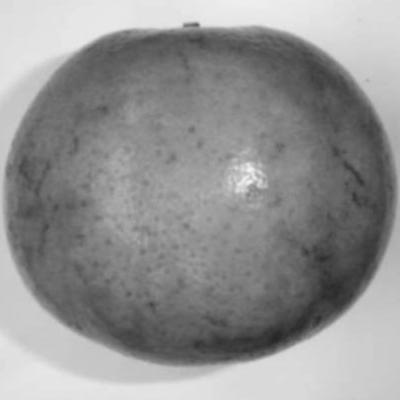
\includegraphics[width=8cm]{tex/choku3.jpg}

\section{Pengolahan Dengan Algoritma}

\subsection{Deteksi Tepi}

Hasil transformasi dengan berbagai skala dan threshold untuk deteksi tepi.

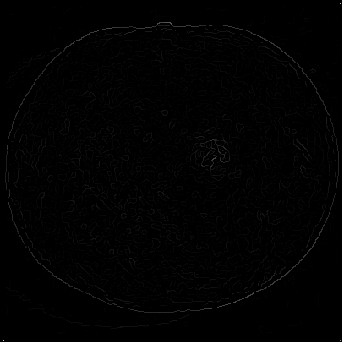
\includegraphics[width=8cm]{tex/canny2.png}

Berdasarkan pengamatan maka skala=x menghasilkan tepi yang paling tajam.

Untuk tepi yang menunjukkan batas antara daerah cacat dengan daerah normal dilakukan \emph{thresholding} pada nilai \emph{magnitude of gradient}.

(Hasil setelah threshold)

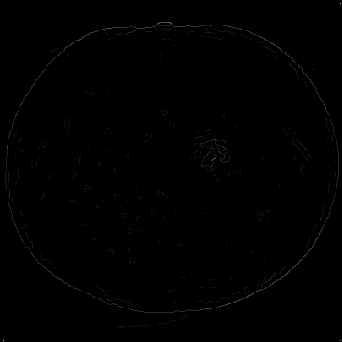
\includegraphics[width=8cm]{tex/canny3.png}

\subsubsection{Penentuan Region}

Selanjutnya dilakukan operasi \emph{flood fill}. Diambil satu titik pada tiap daerah yang dibatasi oleh tepi, jika titik tersebut mempunyai nilai intensitas permukaan tidak normal, lakukan flood fill. Hasil akhir tahap ini adalah mask yang menunjukkan daerah-daerah cacat pada kulit jeruk.

\section{Interpretasi Hasil}

Data menunjukkan bahwa algoritma deteksi tepi Canny dapat menentukan batas-batas permukaan kulit jeruk yang cacat. Akurasi deteksi daerah cacat ditentukan oleh posisi daerah cacat yang mempengaruhi kontras citra kulit jeruk. Akurasi pada bagian \ldots adalah \ldots sementara untuk bagian \ldots adalah \ldots.

Karena metode yang digunakan mengacu pada tepi daerah cacat maka akurasi metode tidak diukur dari prosentase kesalahan luas cacat yang terdeteksi namun dari banyaknya daerah-daerah cacat yang terdeteksi dan ketepatan lokasi deteksi tersebut.

(confusion matrix, presisi, akurasi)

\end{document}
